% appendix.tex
\documentclass[dareport.tex]{subfiles}
\begin{document}
% Content here
\section{Appendix}


\begin{figure}[h]
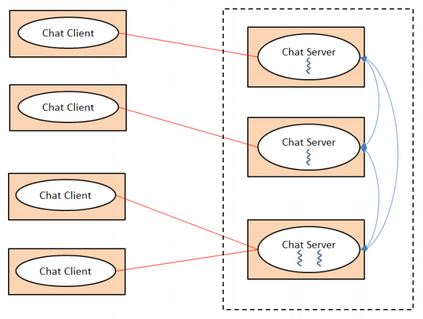
\includegraphics[scale=0.9]{strike_architecture.jpg}
\centering
\caption{Basic Strike Architecture}
\label{fig:strike_arch}
\centering
\end{figure}

%\begin{figure}[!tbp]
%  \centering
%  \begin{minipage}[b]{0.6\textwidth}
%    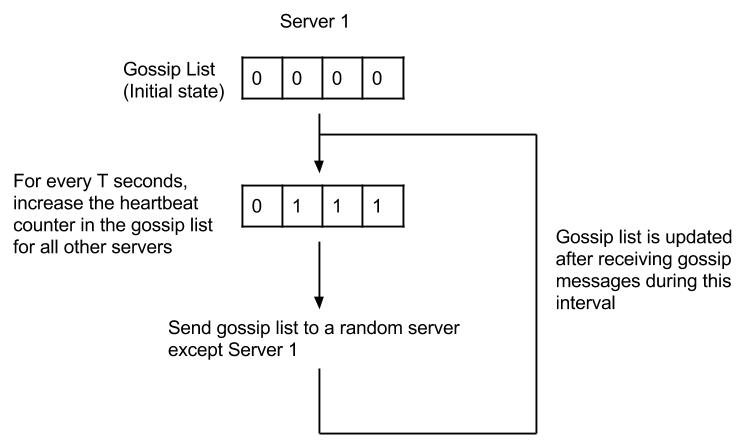
\includegraphics[width=\textwidth]{gossip_send.jpg}
%    \caption{Sending Gossip Message}
%  \end{minipage}
%  \hfill
%  \begin{minipage}[b]{0.6\textwidth}
%    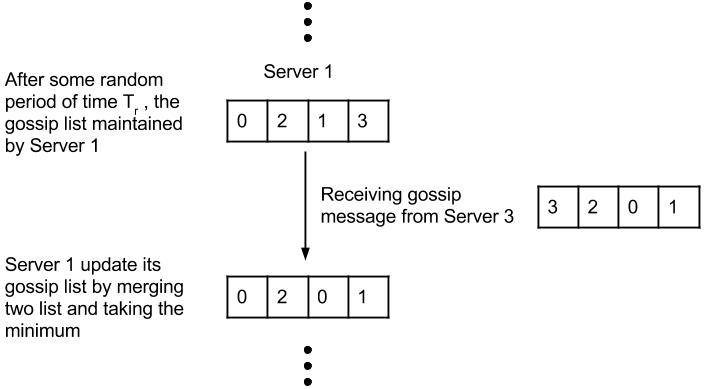
\includegraphics[width=\textwidth]{gossip_receive.jpg}
%    \caption{Updating Gossip List}
%  \end{minipage}
%\end{figure}

%\begin{figure}[h]
%\centering
%\begin{minipage}{.7\textwidth}
%  %\centering
%  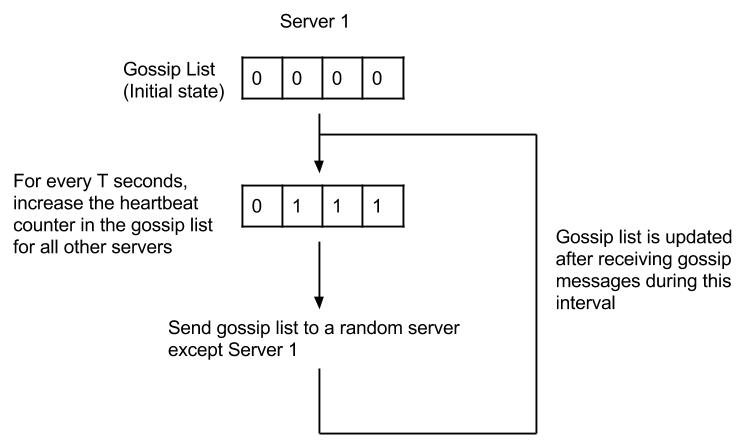
\includegraphics[width=.8\linewidth]{gossip_send.jpg}
%  %\captionof{figure}{A figure}
%  \label{fig:test1}
%\end{minipage}%
%\begin{minipage}{.7\textwidth}
%  %\centering
%  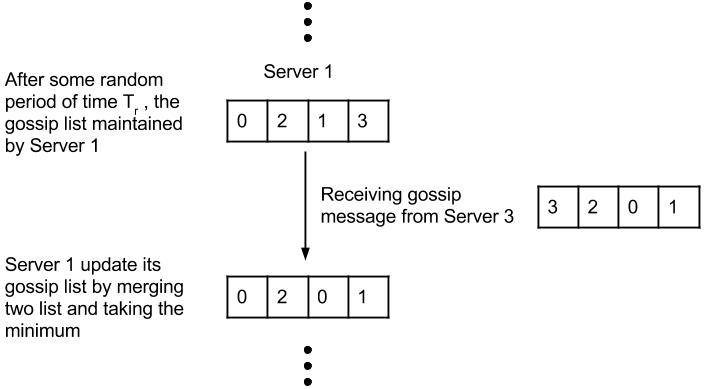
\includegraphics[width=.8\linewidth]{gossip_receive.jpg}
%  %\captionof{figure}{Another figure}
%  \label{fig:test2}
%\end{minipage}
%\end{figure}


\begin{figure}[h]
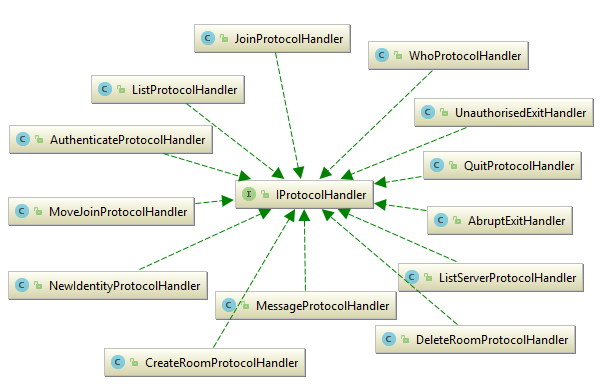
\includegraphics[scale=0.9]{strike_protocol_handlers.png}
\centering
\caption{Strike Server - Protocol Handlers}
\label{fig:protohdl}
\centering
\end{figure}

\begin{figure}[h]
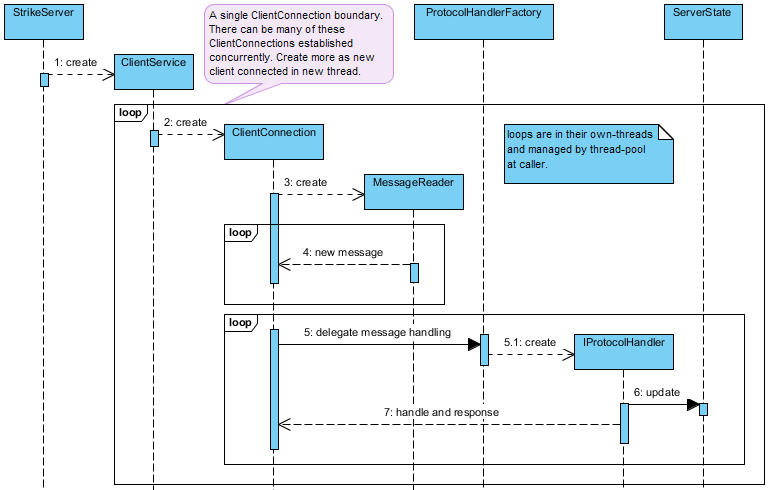
\includegraphics[scale=0.9]{strike_server_client_conn.png}
\caption{Strike Server - Client Connection Sequence Diagram}
\label{fig:clientsq}
\centering
\end{figure}

\begin{figure}[h]
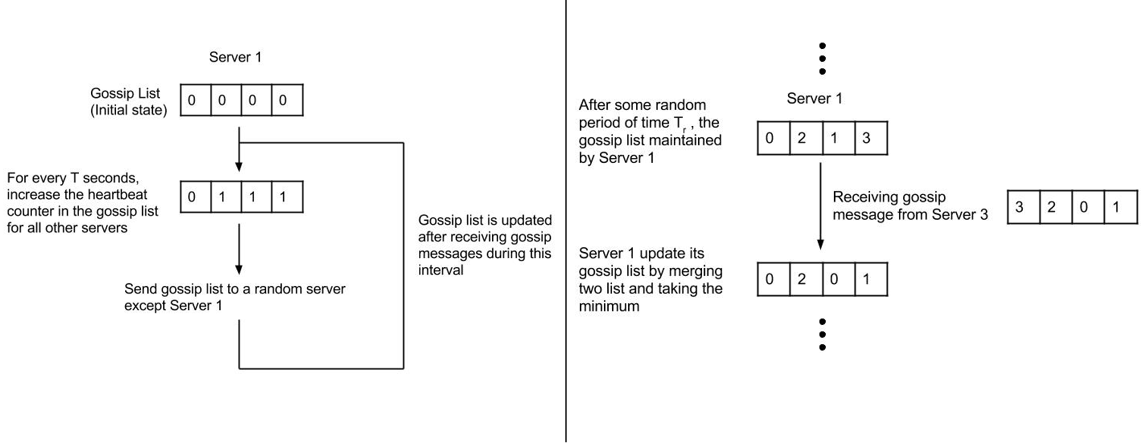
\includegraphics[scale=0.62]{gossip_send_receive.png}
\centering
\caption{Sending and Receiving Gossip Message}
\label{fig:send_receive_gmsg}
\centering
\end{figure}

%\begin{figure}[h]
%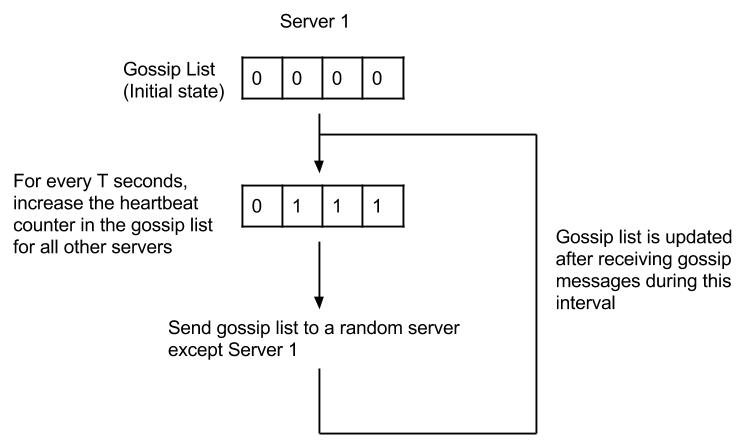
\includegraphics[scale=0.35]{gossip_send.jpg}
%%\centering
%%\caption{Gossip Module - Sending Gossip Message}
%\caption{Sending Gossip Message}
%\label{fig:sending_gmsg}
%\centering
%\end{figure}
%
%\begin{figure}[h]
%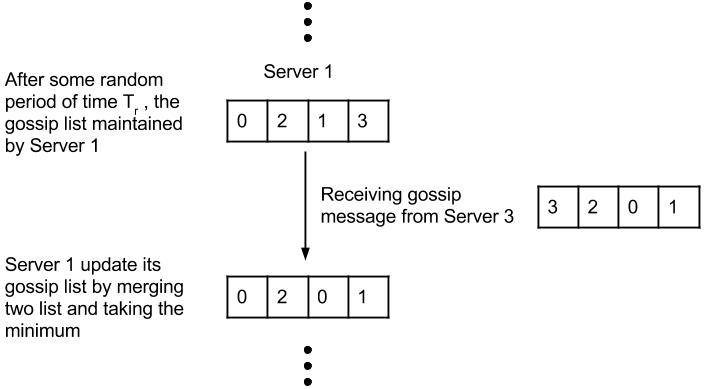
\includegraphics[scale=0.35]{gossip_receive.jpg}
%%\centering
%%\caption{Gossip Module - Receiving Gossip Message and Updating Gossip List}
%\caption{Updating Gossip List}
%\label{fig:receiving_gmsg}
%\centering
%\end{figure}


% Election

\clearpage

\begin{algorithm}[H]
	\small
	\caption{Bully Election Algorithm}
	\label{bully-algorithm}
	\begin{algorithmic}[1]
		\BState \emph{BEGIN}
		\Procedure{StartElection}{$P_{i}$}
		\For {every process $P_{j} : priority(P_{j}) > priority(P_{i}$)}
			\State $P_{i}$ sends \emph{election} message to $P_{j}$
		\EndFor
		\State $P_{i}$ waits for \emph{answer} message for the interval T2.
		\If {no \emph{answer} message within timeout T2}
		
		\Comment No process with priority higher than $P_{i}$ exists.
		
		\Comment $P_{i}$ is the coordinator.
			\For {every process $P_{j} : priority(P_{j}) < priority(P_{i}$)}
				\State $P_{i}$ sends \emph{coordinator} message to $P_{j}$
			\EndFor
			\State $P_{i}$ stops election procedure.
		\Else
		
		\Comment A higher priority process has replied.
			\State $P_{i}$ waits for \emph{coordinator} message for the interval T3.
		\If {$P_{i}$ receives \emph{coordinator} message from $P_{j}$ within timeout T3}
		
		\Comment A higher priority process has elected itself as the leader.
			\State $P_{i}$ admits $P_{j}$ as the new coordinator.
			\State $P_{i}$ stops election procedure.
		\Else
			\State \textproc{StartElection($P_{i}$)}
			\Comment $P_{i}$ restarts the election
		\EndIf
		\EndIf
		\EndProcedure
		\State A process $P_{i}$ does not receive a response within T1 from the coordinator.
		
		\Comment Current coordinator has failed.
		\State\indent \textproc{StartElection($P_{i}$)}
		\State A process $P_{j} \left[priority(j) > priority(i)\right]$ receives an \emph{election} message from $P_{i}$
		\State\indent $P_{j}$ sends an \emph{answer} message to $P_{i}$
		\State\indent \textproc{StartElection($P_{j}$)}
		\State A process $P_{j} \left[priority(j) < priority(i)\right]$ receives a \emph{coordinator} message from $P_{i}$
		
		\Comment A higher priority process has been elected.
		\State\indent $P_{j}$ admits $P_{i}$ as the new coordinator.
		\State\indent $P_{j}$ stops election procedure.
		\BState \emph{END}
	\end{algorithmic}
\end{algorithm}


\begin{algorithm}[H]
	%\small
	\caption{Fast Bully Election Algorithm - Start failure recovery}
	\label{fast-bully-algorithm-start-failure-recovery}
	\begin{algorithmic}[1]
		\BState \emph{BEGIN}
		\Procedure{StartFailureRecovery}{$P_{i}$}
		\State $P_{i}$ sends \emph{iamup} message to every process
		\State $P_{i}$ waits for \emph{view} message for interval T2
		\If{no \emph{view} message within T2}
		
		\Comment $P_{i}$ is the coordinator
		\State Stop the procedure
		\Else
		\State $P_{i}$ compares the received views with its view.
		\If {view of $P_{i}$ $\ne$ receieved view}
			\State $P_{i}$ updates its view.
		\EndIf
		\If {$priorty(P_{i}) > priority(P_{j})$ $\forall P_{j}$ in its view}
		
		\Comment $P_{i}$ is the highest priority process in the current network.
			\For {every process $P_{j} : priority(P_{j}) < priority(P_{i}$)}
				\State $P_{i}$ sends \emph{coordinator} message to $P_{j}$
				\State $P_{i}$ stops the procedure.
			\EndFor
		\Else
			\State $P_{i}$ admits the highest priority process in its view as the coordinator.
			\State $P_{i}$ stops the procedure.
		\EndIf
		\EndIf
		\EndProcedure
		\BState \emph{END}
	\end{algorithmic}
\end{algorithm}


\begin{algorithm}
	%\small
	\caption{Fast Bully Election Algorithm -  Start election}
	\label{fast-bully-algorithm-start-election}
	\begin{algorithmic}[1]
		\BState \emph{BEGIN}
		\Procedure{StartElection}{$P_{i}$}
			\For {every process $P_{j} : priority(P_{j}) > priority(P_{i}$)}
				\State $P_{i}$ sends \emph{election} message to $P_{j}$
			\EndFor
			\State $P_{i}$ waits for \emph{answer} message for the interval T2.
			\If {no \emph{answer} message within timeout T2}
				
			\Comment No process with priority higher than $P_{i}$ exists.
				
			\Comment $P_{i}$ is the coordinator.
				\For {every process $P_{j} : priority(P_{j}) < priority(P_{i}$)}
					\State $P_{i}$ sends \emph{coordinator} message to $P_{j}$
				\EndFor
				\State $P_{i}$ stops election procedure.
			\Else
			
			\Comment Processes with higher priority have answered.
				\State add answered process to answered list.
				\State send \emph{nomination} message to $P_{j}$ : $priority(P_{j}) > priority(P_{k})$ $\forall P_{k}$ that answered  $P_{i}$ \label{send-nomination}
				\State $P_{i}$ waits for \emph{coordinator} message for interval T3.
				\If {A coordinator message from $P_{j}$ is received}
					\State $P_{i}$ admits $P_{j}$ as the new coordinator.
					\State $P_{i}$ stops election procedure.
				\Else
					\State Remove $P_{j}$ from answered list.
					\State Repeat \cref{send-nomination} for the next $P_{j}$ in the answered list.
					\If {Answered list is empty}
						\State \textproc{StartElection($P_{j}$)}
					\EndIf
				\EndIf
			\EndIf
		\EndProcedure
		\BState \emph{END}
	\end{algorithmic}
\end{algorithm}


\begin{algorithm}
	%\small
	\caption{Fast Bully Election Algorithm}
	\label{fast-bully-algorithm}
	\begin{algorithmic}[1]
		\BState \emph{BEGIN}
		\State A process $P_{i}$ recovers from failure
			\State\indent\textproc{StartFailureRecovery($P_{i}$)}
		\State A process $P_{i}$ may receive an IamUp message from $P_{j}$
			\State\indent $P_{i}$ sends view message to $P_{j}$.
		\State A process $P_{i}$ does not receive a response within T1 from the coordinator
			\State\indent\textproc{StartElection($P_{i}$)}
		\State A process $P_{j} \left[priority(j) > priority(i)\right]$ receives an \emph{election} message from $P_{i}$
			\State\indent $P_{j}$ sends an \emph{answer} message to process $P_{i}$
			\State\indent $P_{j}$ waits for either a \emph{coordinator} or a \emph{nomination} message for interval T4
			\State\indent {\textbf{if} no \emph{coordinator} or \emph{nomination} message within T4 \textbf{then}}
				\State\indent\indent\textproc{StartElection($P_{j}$)}
			
			\State { A process $P_{j} \left[priority(j) > priority(i)\right]$ receives a \emph{nomination} message from $P_{i}$}
			
			\Comment The current election manager has decided $P_{j}$ to be the new coordinator\footnote{Current election manager is the process which started the ongoing election}.
				\State\indent $P_{j}$ admits itself as the new coordinator.
				\State\indent {\textbf{for} every process $P_{k} : priority(P_{k}) < priority(P_{j}$) \textbf{do}}
					\State\indent\indent $P_{j}$ sends \emph{coordinator} message to $P_{k}$
					\State\indent\indent $P_{j}$ stops the procedure.
			\State {A process $P_{j} \left[priority(j) < priority(i)\right]$ receives a \emph{coordinator} message from $P_{i}$}
			
			\Comment A higher priority process has been elected.
				\State\indent $P_{j}$ admits $P_{i}$ as the new coordinator.
				\State\indent $P_{j}$ stops election procedure.
		\BState \emph{END}
	\end{algorithmic}
\end{algorithm}

\end{document}